\chapter{Kameragestützten Validierungsprozessen in der Lagerverwaltung}\label{KameragestützteInventur}

Aufgabe der Lagerzelle ist die automatische Ein- und Auslagerung von Bechern mit oder ohne Produkt.
Die Informationen, die dafür übergeben werden oder entstehen, müssen gespeichert werden um bei einer Produktbestellung wieder das korrekte Produkt auszugeben.
Das in \ref{Software} beschriebene Datenmodell erledigt genau das. Wird ein Becher von Ort A nach Ort B bewegt, 
passieren notwendige Änderungen am Datenmodell selbst. Fehler im Datenmodell können durch systematische Tests des relevanten Quellcodes entdeckt und behoben werden. 
Zu diesem Zweck sind die Tests \verb|test\_inventory| und \verb|test_inventoryController| implementiert. 
Die Tests sind jedoch auf das Datenmodell und seinen Controller beschränkt und ein \glq unbefugter\grq Zugriff kann in Python nicht unebdingt verhindert werden. 
Eine weitere Fehlerquelle kann die Möglichkeit der manuellen Überschreibung des Lagerbestands sein oder gar ein manueller Eingriff in der Lagerzelle selbst. 

Um diese Fehler zu erkennen, soll ein kameragestütztes Inventursystem entworfen werden. 
    \section {Konzepte}

    Es werden zwei Konzepte verfolgt.
    Diese dienen dazu jederzeit einen sicheren Betrieb der Lagerzelle zu gewährleisten in dem Sie die Position der Becher und Paletten überprüfen.
    Da es sich bei den Produkten um eine simulierte Getränkeproduktion handelt, können sie nicht so leicht erkannt werden und sind daher nicht Gegenstand dieser Arbeit. 

    \subsection{Anwendungsfall 1: Inventur auf Anforderung}\label{InventurAufAnforderung}

    Eine Kamera ist mittig auf dem Greifer des Roboters montiert. Auf Anforderung des Bedieners fährt der Roboter festgelegte Wegpunkte ab. 
    Bei Erreichen eines Wegpunkts wird ein Signal emittiert und eine definierte Zeit für die Bildaufnahme abgewartet.
    Da die Bilder den Wegpunkten und die Wegpunkte den Lagerstellen zugeordnet sind, kann durch die Erkannten arUco Marker auf die 
    im Lager vorhandenen Paletten und Becher zurückgeschlossen werden. 
    Die Gefahr, dass der Roboter mit einem Hindernis kollidiert, wird dadurch minimiert. 

    \subsection{Anwendungsfall 2: Inventur im laufenden Prozess}\label{InventurImProzess}

    Im laufenden Prozessbetrieb wird der Roboter Becher und Paletten zwischen festgelegte Lagerstellen bewegen.
    Bevor der Roboter aus dem Regal eine Palette entnimmt, wird ein Bild aufgenommen und geprüft, ob die Palette tatsächlich vorhanden ist.
    Genauso wird überprüft, ob der Abstellort tatsächlich frei ist bevor der Roboter eine Palette ablegt.
    Analoge Prüfungen werden für die Becher durchgeführt.

    \subsection{Grundsätzliche Überlegungen}
    Mögliche Lagerorte sind:
    \begin{itemize}
        \item Der mobile Roboter in der Entladestation (Ein Becher). 
        \item Der Kommissionstisch (Zwei Abstellmöglichkeiten für Paletten)
        \item Das Lager (18 mögliche Abstellorte für Paletten)
    \end{itemize}
    Zusätzlich kann ein Becher oder eine Palette temporär von einem Greifer bewegt werden. 
    All Diese Orte sind im Datenmodell und im GUI berücksichtigt. 
    Auf der Steuerung IRC5 des Roboters sind Routinen programmiert, die die jeweiligen Becher/Palettenbewegungen implementieren.
    Sie werden vom \verb|ABBController| aus über den entsprechenden Service via TCP aufgerufen. 
    Ein entsprechendes Signal zur Bildaufzeichnung und Bildauswertung kann erfolgen, wenn der Greifer die Position vor dem Lagerort erreicht hat. 
    Durch den Aufruf der Routine ist festgelegt zu welchem Lagerort das Bild zugeordnet ist.
    Dies ist zu jedem Zeitpunkt eindeutig bestimmt. 

    Damit eine Kamera die Becher und Paletten voneinander unterscheiden kann, müssen an den Bechern und an den Paletten eindeutige optische Marker angebracht sein. 
    Es bringt keinen Mehrwert Paletten voneinander zu unterscheiden, da diese nur den Zweck haben bis zu zwei Becher umfallsicher zu halten. 
    Daher wird an jeder Palette der gleiche Marker angebracht.

    Aus der persönlichen Beobachtung der Lagerzelle reifte die Idee, dass alle Paletten und die vorderen Becher durch eine Übersichtskamera erkannt werden können. 
    Dazu wird eine Kamera mit einer höheren Auflösung in die obere Ecke der Lagerzelle gehängt. 
    Das Regal ist dann in einem kleinen Bildausschnitt im oberen Bildbereich zu sehen. 

    Der Roboter verdeckt dabei in seiner Grundstellung den unteren linken Breich des Regals, sodass die Lagerpositionen L13, L14, L15 nicht erkannt werden können. 
    Die Vermutung liegt nahe, dass die Positionen L14 und L15 auch erkannt werden, wenn der Roboterarm in eine geeignete Position fährt. 

    Um die Robustheit zu erhöhen, muss das Regal automatisch aus dem Bild extrahiert werden. 
    Zu diesem Zweck wird an dem Regal an jeder Ecke und an jedem Regalboden ein arUco Marker angebracht.
    Auf diese Wiese kann die Software automatisch den interessanten Bereich des Bilds Extrahieren. 
    
    
    \section {Auswahl der optischen Marker}

    Die Arbeit von \cite[Sebastian Hübler]{Hübler2019} legt die Verwendung von arUco Markern nahe. 
    Laut seiner Arbeit werden die Marker auch dann noch erkannt, wenn der vom Kamerahersteller angegebene Mindestabstand unterschritten wird und das Bild unscharf ist. 
    Die Marker sind quadratisch, haben einen umlaufenden Rand und eine mittige Binärmatrix. 
    Über die Binärmatrix kann wie bereits in \ref{arucoMarker} beschrieben, auch die Orientierung des Markers ermittelt werden.
    Da jede Binärmatrix einen Integerwert darstellt, ist die Anzahl der einzigartigen ID's aus den Binärmatritzen proportional zu ihrer Kantenlänge.
    Die ID entspricht dabei nicht der Binärzahl die etwa aus der Matrix dekodiert werden könnte, sondern die Marker sind in der \cite[OpenCV]{OpenCVaruco} Bibliothek in
    Dictionarys organisiert. Die ID entspricht dem Index des Markers im Dictionary.

    Als Marker werden jene aus dem Dictionary \verb|6x6-250| verwendet. Das bedeutet, dass die Marker eine Kantenlänge von 6 Bits haben und eine Markergröße von 250 Pixel.

    \section {Auswahl der Kameras, Objektive und Aufstellung}

    Die Auswahl der Kameras beruht auf meiner \cite[Semesterarbeit]{Semesterarbeit}. 
    Die ausgewählten Kameras sind Industriekameras der Firma IDS GmbH und haben keine Optik. 
    Daher erfolgt anhand des kleinsten zu erwartenden Details, des Bildbereichs sowie der Kameraparameter (Brennweite und Sensorgröße) eine Objektivauswahl. 

    Für die Übersichtskamera wurde das Objektiv auf den größtmöglichen Schärfebereich eingestellt, sodass die Chance besteht eine Markererkennung sowohl im Regal als auch im Kommissionstisch vorzunehmen. 

    ----

    Die ursprüngliche $\mu$Eye Kamera erweist sich mit Objektiv zu lang, um sie an dem Greifer zu montieren ohne die Kollisionsgefahr zu erhöhen. 
    Sie müsste exzentrisch auf dem Griefer montiert werden und würde somit nicht mehr orthogonal zu den Markern stehen.
    Aus diesem Grund wird eine ESP32 Kamera mit verbauter Optik verwendet.
    Sie ist wesentlich kleiner und kann direkt auf den Greifer montiert werden.
    Der Mindestabstand zwischen Kamera und Objekt ist vom Hersteller nicht angegeben, die Aufnahmen aus dem Kapitel \ref{ErkennungsrateESP32} 
    zeigen aber sehr gute Ergebnisse.
    Die ESP32 Kamera hat einen eingebauten Webserver, über dessen RESTful API die aufgenommenen Bilder heruntergeladen werden können. 
    Die Kamera kann von ihren Abmaßen direkt auf den Greifer montiert werden und der angegebene Mindestabstand für die Appertur wird dabei nur knapp unterschritten. 
    Testaufnahmen zeigen, dass die Marker bei gegebenen Abstandsverhältnissen noch scharf abgebildet werden. 

    \begin{figure}
        \caption[Optische Verzerrung der Übersichtskamera]
        {\small bei diesem Bild wurde eine Markererkennung mit dem OpenCV Paket durchgeführt, Aus den maximalen und minimalen Koordinaten wurde ein grünes Rechteck erstellt. Aus den 4 Markern der rechten Seite und den 2 Markern links wurde der Verlauf der vertikalen Regalkanten ermittelt und das Bild so gedreht, dass die rechte Seite vertikal ist.}\label{fig:figure10}
        \includegraphics[width = \textwidth ]{Bilder/verzerrtesBild.png}
        \centering
    \end{figure}

    \section {Perspektivische Korrektur}

    Wie in dem Bild \ref{fig:figure10} zu sehen, ist das Regal perspektivisch stark verzerrt.
    Der Verzerrung durch die Linse wird vor Allem durch die horizontale Linie deutlich, nachdem das Bild so gedreht wurde, dass der rechte Regalrand vertikal ist. 
    Für die Erkennung der Marker und der Bildsegmentierung für die Zuordnung der Marker zu den Lagerorten ist es also erforderlich entweder eine geometrische Kalibrierung der Appertur vorzunehmen oder das Bild im interessierenden Bereich zu rektifizieren. 
    Eine 4-Punkt Entzerrung ist aufgrund des geringen Aufwands und der hohen Auflösung der gewählte Weg. 
    Um die Rektifizierung zu automatisieren, wurden die oberen Regalecken und die Kreuzungen der Regalböden mit dem äußeren Rahmen mit identischen arUco Marker versehen. 
    Die obere linke Regalecke ist nicht im Bildbereich und der dortige Marker kann somit nicht erkannt werden. 
    Als die Für die 4-Punkt Entzerrung notwendigen Punkte werden die Schnittpunkte der beiden oberen Regalböden mit dem Außenrand des Regals gewählt. 
    Die eigentliche Rektifizierung ist Teil des \verb|stocktaking| Service der Software und nutzt dazu die Methoden des \verb|skimage| Pakets in Python.

    \begin{figure}
        \caption[Ablauf Bildverarbeitung und Markererkennung der Übersichtskamera]
        {\small Ablauf Bildverarbeitung und Markererkennung der Übersichtskamera. Die ursprüngliche Aufnahme wird dupliziert. Der obere Pfad zeigt die Ermittlung der Transformationsdaten mithilfe der Regalmarker. Im Unteren PFad wird das Originalbild rektifiziert und segmentiert bevor Paletten und Becher-ID's extrahiert werden.}\label{fig:figure11}
        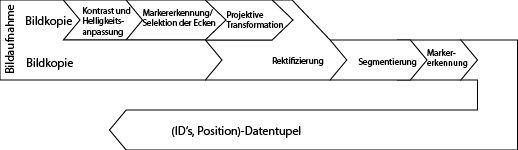
\includegraphics[width = \textwidth ]{Bilder/AblaufErkennungSellCam.png}
        \centering
    \end{figure}

    Für die perspektivische Entzerrung wird das Python Paket \verb|skimage| verwendet. Der Name steht für \glq \textbf{S}cience \textbf{K}it for \textbf{Image}processing \grq.
    Das Untermodul \verb|util.transform| enthält eine Klasse \verb|ProjectiveTransform|. Die \verb|estimate| Methode dieser Klasse akzeptiert als Parameter zwei Matritzen \verb|src| und \verb|dst| und ermittelt eine Transformationsmatrix.
    Als \verb|src| werden die Bildkoordinaten der 4 Marker angegeben und als dst die \glq realen \grq Koordinaten.
    Die \verb|warp| Methode akzeptiert neben der Instanz der o.g. Klasse auch die Eingabe- und Ausgabedimensionen.     
    
    Versuche haben gezeigt, dass die Erkennungsrate der Regalmarker deutlich verbessert werden kann, wenn vor der Markererkennung die Helligkeit und der Kontrast angepasst werden. 
    Noch dazu tritt eine deutliche Verbesserung der Erkennungsrate ein, wenn das Bild etwas überbelichtet ist. 
    Leider sind die Erkennungsraten der Paletten/Becher deutlich schlechter, wenn das angepasste Bild verwendet wird, welches für die Erkennung der Regalmarker optimiert ist. 
    Die Lichtverhältnisse der einzelnen Lagerplätze sind unterschiedlich, weshalb es naheliegt den Kontrast und die Helligkeit der einzelnen Bildbereiche anzupassen. 
    Dafür wird nach der Bildaufnahme das Bild mit der \verb|copy| Funktion des \verb|numpy| Pakets dupliziert.

    Nach der Transformation des Bildes, wird das originale Bild auf die relevanten Bereiche zugeschnitten und in die jeweiligen Lagerbereiche segmentiert.
    Die einzelnen Lagerbereiche \glqq sections \grqq werden danach noch mal zwischen Palette und Becher Bereiche getrennt. 
    Danach erfolgt erneut eine Helligkeits und Kontrastanpassung bevor die einzelnen Marker in den Bildsegmenten bestimmt werden. 
    Die Bildsegmente und die erkannten Marker mit ihren ID's werden in entsprechenden Listen des \verb|stocktaking| Services gespeichert.

    \section {Automatische Kontrast und Helligkeitsanpassung}
    Der Algorhythmus ist in der Methode \verb|_automatic_brightness_and_contrast| des \verb|stocktaking| Services implementiert. 

    Die Methode bekommt als Argumente ein Bild oder Bildausschnitt als Graustufenbild, welches mit der Bildklasse des \verb|cv2| paket (OpenCV) identisch ist. 

    Außerdem wird ein Wert übergeben, der als Prozentwert interpretiert wird, nachfolgend als $n$ bezeichnet.
    
    Ziel des Algorhytmus ist es, das ursprüngliche Histogramm des Bildes auf das $\frac{n}{2}$-te bis $\frac{(100-n)}{2}$-te Prozentil zu beschränken und
    daraus eine neue Histogrammverteilung zu berechnen. 

    Die Berechnung des neuen Histogramms erfolgt mit der Funktion aus der Bibliothek OpenCV \verb|convertScaleAbs()|. 
    Die Funktion benötigt als Argumente einen Inputarray sowie einen Skalierungsfaktor $\alpha$ und einen Wert $\beta$, der zu den Histogrammwerten addiert wird.
    Die Funktion gibt das angepasste Bild zurück.
    Kernproblem ist also die Bestimmung der beiden Parameter $\alpha$ und $\beta$. 

    Die zusammengefassten Schritte des Algorhythmus sind:
    \begin{enumerate}
        \item Von dem übergebenen Bildausschnitt wird ein Histogramm der Graustufenskala mit einer Auflösung von 8 Bit berechnet. Dazu wird die Funktion \verb|cv2.calcHist()| verwendet.
        \item Die kumulative Verteilung des Histogramms wird berechnet.
        \item Der minimale Grauwert des neuen Histogramms wird mit $g_{min} = 0$ initialisiert. Er wird in einer Schleife erhöht, solange das $\frac{n}{2}$-te Prozentil der kumulativen Verteilung nicht überschritten ist.
        \item Der maximale Grauwert des neuen Histogramms wird mit $g_{max} = 255$ initialisiert. Er wird in einer Schleife reduziert, solange das $\frac{(100-n)}{2}$-te Prozentil der kumulativen Verteilung nicht unterschritten ist.
        \item Der Skalierungsfaktor $\alpha$ wird mit $\alpha = \frac{255}{g_{max} - g_{min}}$ berechnet.
        \item Der additive Wert $\beta$ wird mit $\beta = -\alpha \cdot g_{min}$ berechnet.
        \item Mit den berechneten Werten für $\alpha$ und $\beta$ wird die \verb|cv2.convertScaleAbs()| Funktion ausgeführt. Der Rückgabewert ist das angepasste Bild.
    \end{enumerate}

    Für den Prozentsatz der Abschneidung des Histograms wurde $n=2$ gewählt. Da der Wert sich als robust erwies, habe ich diesen Wert nicht weiter optimiert.
    Der Algorythmus ist in Anlehnung an die Diskussion auf dem Internetforum Stackoverflow \cite{SOcontrast} entstanden. 
    Wird der Code 1:1 übernommen, erhält man beim Ausführen DeprecationWarnings. Der Code musste daher an die Python 3.11 Version angepasst werden. 
    
    \clearpage
    \lstinputlisting[language=Python, caption=Automatische Helligkeits und Kontrastanpassung, label=calcBrightContrast]{Listings/automatic_brightness_and_contrast.py}
    \clearpage

    \section {Markererkennung}

    Für die Erkennung der optischen arUco Marker wird aus der OpenCV Bibliothek das Modul \verb|aruco| benutzt. 
    Die Erkennung erfolgt über die Funktion \verb|detectMarkers|, die als Argumente ein Graubild oder Bildausschnitt sowie ein arUco Dictionary übergeben bekommt.
    Der vereinfachte Algorhythmus ist in \ref{arucoMarker} beschrieben. Die dabei verwendeten Parameter sind in \cite{OpenCVaruco} beschrieben.
    
    Der Erfolg der Erkennung der Marker hängt demnach unter Anderem davon ab, dass die einzelnen Bits in der Binärmatrix ähnlich breit sind. 
    Der Algorithmus zum Erkennen der Marker benutzt für die einzelnen Schritte insgesamt 31 Parameter, die viele Aspekte der Erkennung beeinflussen.
    Die Standardeinstellungen sind für Bilder / Bildsegmente moderater Größe eine sinnvolle Wahl. 
    
    Laut \cite[OpenCV]{OpenCVaruco} ist die Erkennung robust gegenüber Rotation und Perspektivischer Verzerrung. 
    Die Erkennung versagt allerdings, wenn wie z.B. in \ref{fig:figure20} der Marker durch eine Wölbung verzerrt wird, die in diesem Falle durch die 4-Punkt Verzerrung überlagert ist.
    In dem Bild ist deutlich zu erkennen, dass die Bits im rechten Bereich deutlich breiter als im linken Bereich sind. 
    Dies ist Anlass zum nächsten Abschnitt \ref{ChapBildmatrixanalyse}.

    \subsection{Bildmatrixanalyse an einem gewölbten Marker}\label{ChapBildmatrixanalyse}

    In \ref{fig:figure21} ist die Binärmatrix eines durch die Wölbung verzerrten Markers dargestellt. 
    In \ref{Bildmatrixanalyse} ist das Script abgedruckt mit dem die Abbildung erzeugt wurde.

    Das Bildsegment, das den Bechermarker abbildet wird grob auf die Außenmaße des Markers zugeschnitten.

    Mit der Schwellenwert-Funktion wird das Graubildsegment zu einem binärwertigen Bild umgewandelt.

    Durch die vorangegangene Helligkeits- und Kontrastanpassung \ref{calcBrightContrast}, können die Grenzen dafür sehr eng gefasst werden.
    
    In den zwei Listen \verb|horizontals| und \verb|verticals| sind die x- bzw. y- Koordinaten der Bitmatrix angegeben. 
    Die Koordinaten der beiden Listen sind manuell ermittelt, und zwar so, dass die Linien der Bitgrenzen immer links bzw. unterhalb der Bitgrenze liegen.

    Die Linien der Bitgrenzen werden mittels einer for-Schleife gezeichnet. 
    Ist der Wert des aktuellen Pixels schwarz (also alle Farbkanäle sind 0), wird der Pixel übersprungen, ansonsten wird der Pixel auf die angegebene Farbe gesetzt. 
    Dadurch entsteht der Eindruck, dass die Linien hinter dem Marker verlaufen und die Erscheinung des Markers wird nicht gestört. 
    
    In dem mittleren Subplot sind die Koordinaten der Linien der Bitmatrix über den resultierenden Bits aufgetragen. 
    Ein Bit ist dabei das eingeschlossene Rechteck zwischen der jeweilgen x- bzw. y- Linie. 
    Außerdem wurde für jeden Plot ein ausgleichspolynom geschätzt, um die unterschiedlichen Verläufe zu zeigen. 
    
    Im rechten Subplot ist die Änderung der Pixelbreite eines Bits in x- bzw. y- Richtung über die Bitnummer aufgetragen.
    Hier zeigt sich, dass in der y-Richtung - bis auf einen Ausreißer - keine Änderung der Bitbreite auftritt. 
    
    In x-Richtung ändert sich die Breite der Bits jedoch deutlich.
    Beides wird mit je einem Ausgleichspolynom dargestellt. 
    Hier ist anzumerken, dass der jeweils erste Datentupel (0,0) nicht für das Ausgleichspolynom verwendet wurde. 

    Wie in dem Abschnitt zu arUco Markern \ref{arucoMarker} beschrieben, dient der Rand eines Markers zur Bestimmung der Bitgröße in Pixeln.
    Vergleicht man den Marker mit dem aus dem resultierenden Gitter, ist es nicht verwunderlich, dass die Erkennung fehlschlägt.

    Die y-Indizes der horizontalen Markerlinien ist nicht über die volle Breite des Markers konstant. 
    Die Verzerrung in Folge der Zylinderwölbung des Bechers und der vorangegangenen 4-Punkt Entzerrung stellt somit einen der wenigen Fälle dar, 
    die der sonst so robuste Erkennungsalgorithmus nicht bewältigen kann.

    Auch wenn die Verzerrung einen systematischen Charakter hat, ist sie Abhängig von
    \begin{itemize}
        \item der Position der Übersichtskamera und damit dem Bildbereich
        \item der Position des Bechers in der Lagerzelle
        \item der Position des Bechers in der Palette (vorne / hinten)
        \item der 4-Punkt Entzerrung
        \item dem Verdrehwinkel des Markers entlang der Becherachse zur Kamera.
    \end{itemize}

    Eine Korrekturfunktion zur Reparatur des Markers müsste somit an die jeweiligen Unwägbarkeiten individuell angepasst sein.
    Daher wird davon in dieser Arbeit abgesehen. 
    Selbst wenn eine derartige Funktion implementiert würde, könnten maximal die Becher in der vorderen Reihe der Paletten erkannt werden.
    Die hinteren Plätze sind zu sehr durch die vorderen Becher verdeckt.

    \begin{figure}
        \caption[Bildaufnahme aus der Lagerzelle von der Übersichtskamera.]
        {\small Die Abbildung zeigt die Aufnahme der Kamera und Apertur ohne weitere Bildverarbeitung außerhalb der Kamera. Die leichte Überbelichtung begünstigt das Erkennen der Regalmarker.}\label{fig:figure12}
        \includegraphics[width = \textwidth]{Bilder/LZIP_raw_shot.png}
        \centering
    \end{figure}

    \begin{figure}
        \caption[Bildaufnahme aus der Lagerzelle nach der Kontrastanpassung.]
        {\small Die Aufnahme aus Bild \ref{fig:figure12} nach der automatischen Helligkeits- und Kontrastanpassung.}\label{fig:figure13}
        \includegraphics[width = \textwidth]{Bilder/LZ_Kontrastanpassung.png}
        \centering
    \end{figure}

    \begin{figure}
        \caption[Bild aus der Lagerzelle nach der Rektifizierung und Zuschnitt auf relevanten Regalbereich]
        {\small Die Aufnahme aus Bild \ref{fig:figure12} nach der Kontrastanpassung und Rektifizierung. Im Vordergrund sind die Paletten und Becher gut zu erkennen. Die Becher in der zweiten Reihe sind jedoch deutlich verzerrt.}\label{fig:figure14}
        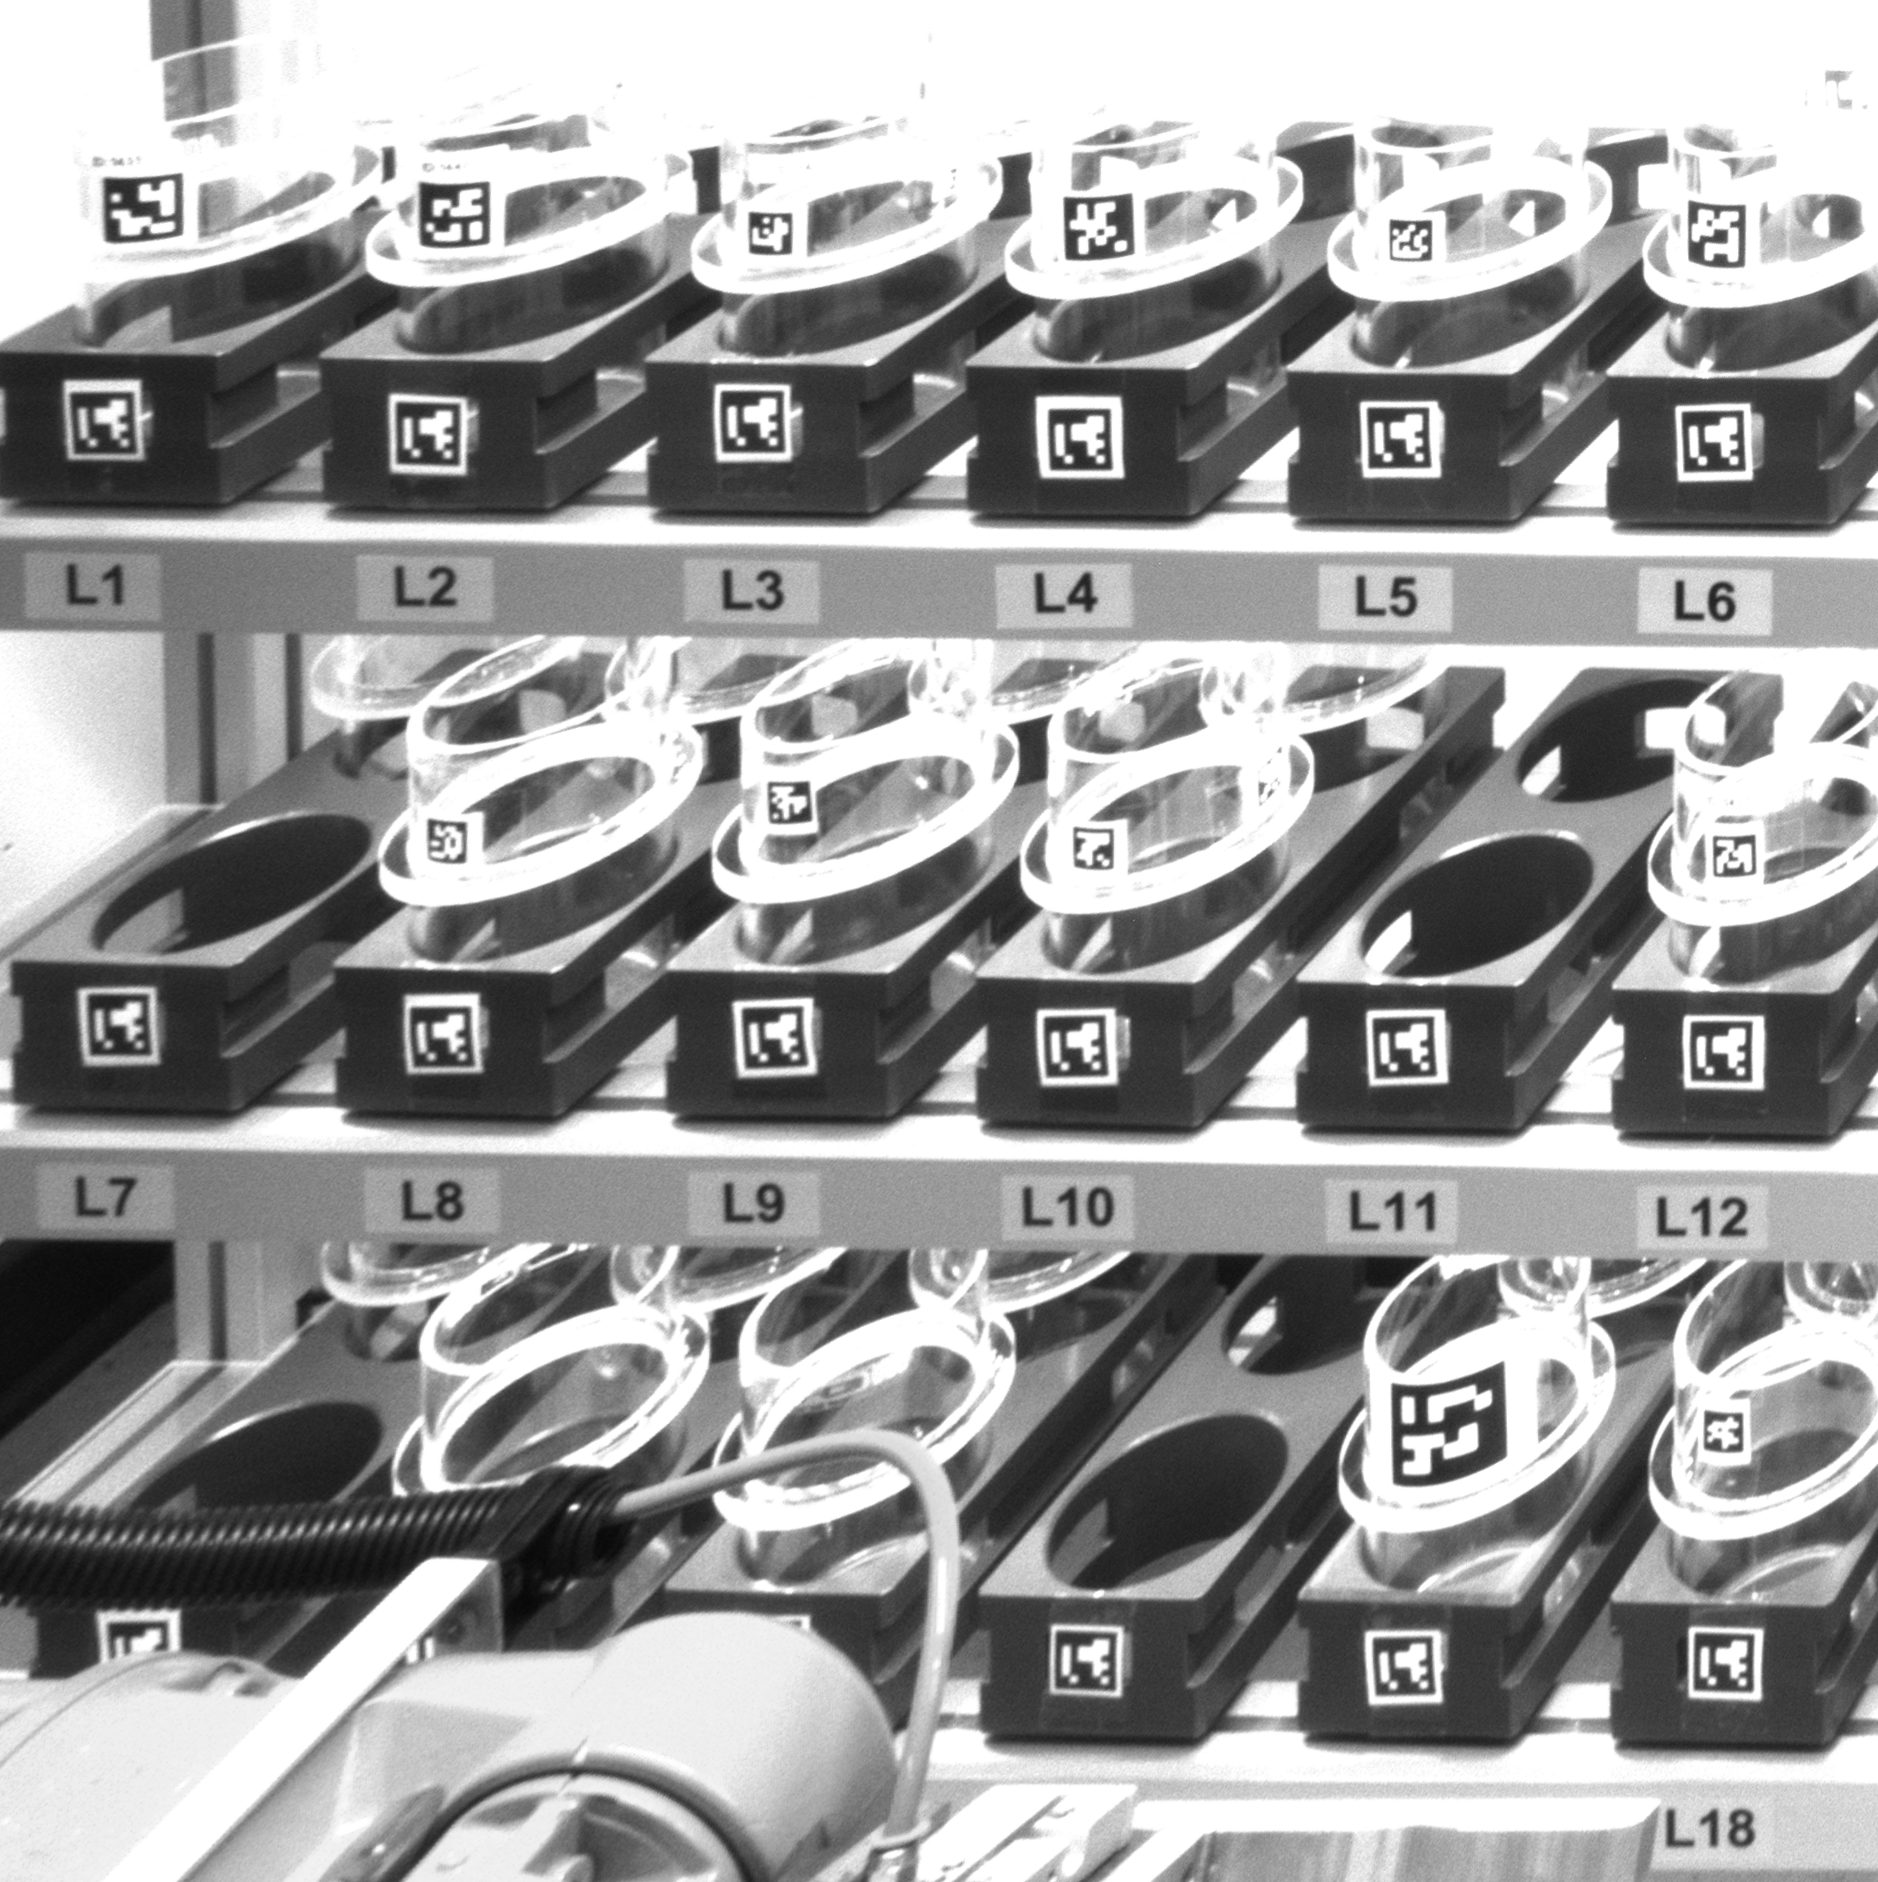
\includegraphics[width = \textwidth]{Bilder/LZ_transformed.png}
        \centering
    \end{figure}

    \begin{figure}
        \caption[Bildzuschnitt auf einen Lagerplatz.]
        {\small Bildzuschnitt einer Lagersektion und weitere Unterteilung in die Bereiche für Becher und Palette. Der Bildausschnitt zeigt einen Lagerslot mit Palette aber ohne Becher im vorderen Lagerslot, der aus \ref{fig:figure15} extrahiert wurde. Der Marker hat kein weißes Rechteck um sich was bedeutet, dass dieser Marker nicht erkannt wurde. Dies liegt vermutlich an der durch die Wölbung gestörten Binärmatrix}\label{fig:figure15}
        \includegraphics*[width = \textwidth/3]{Bilder/section_16.png}
        \centering
    \end{figure}

    \begin{figure}
        \caption[Bildzuschnitt einer Lagersektion und weitere Unterteilung in die Bereiche für Becher und Palette.]
        {\small Der Bildausschnitt zeigt einen Lagerslot mit Palette und Becher im vorderen Lagerslot, der aus \ref{fig:figure15} extrahiert wurde. Der Marker hat kein weißes Rechteck um sich was bedeutet, dass dieser Marker nicht erkannt wurde}\label{fig:figure18}
        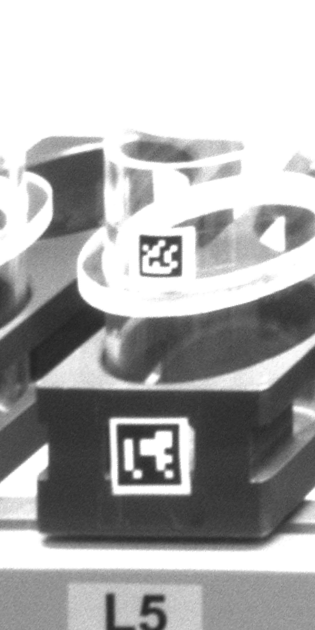
\includegraphics[width = \textwidth/3]{Bilder/section_5.png}
        \centering
    \end{figure}

    \begin{figure}
        \caption[Bild aus der Lagerzelle nach der Rektifizierung und Zuschnitt auf einen Bereich einer Palette]
        {\small Bereich einer Palette, aus \ref{fig:figure14} extrahiert. Der dicke weiße Rahmen wird im Programmcode erzeugt wenn der Marker erfolgreich erkannt wurde. }\label{fig:figure16}
        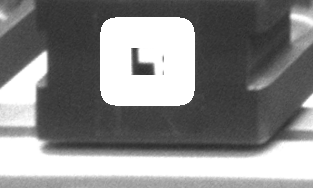
\includegraphics[width = \textwidth/3]{Bilder/pallet_5.png}
        \centering
    \end{figure}

    \begin{figure}
        \caption[Bild aus der Lagerzelle nach der Rektifizierung und Zuschnitt auf einen Bereich einer Palette]
        {\small Bereich einer Palette, aus \ref{fig:figure14} extrahiert. Im Gegensatz zu \ref{fig:figure16} wurde der Marker nicht erkannt. }\label{fig:figure19}
        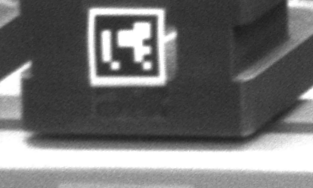
\includegraphics[width = \textwidth/3]{Bilder/pallet_3.png}
        \centering
    \end{figure}

    \begin{figure}
        \caption[Bild aus der Lagerzelle nach der Rektifizierung und Zuschnitt auf einen Bereich eines Bechers]
        {\small Bereich eines Bechers, aus \ref{fig:figure14} extrahiert. Deutlich sichtbar ist die durch die Wölbung des Bechers gestörte Binärmatrix des Markers.}\label{fig:figure17}
        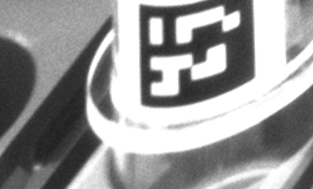
\includegraphics[width = \textwidth/3]{Bilder/cup17.png}
        \centering
    \end{figure}

    \begin{figure}
        \caption[Bild aus der Lagerzelle nach der Rektifizierung und Zuschnitt auf einen Bereich eines Bechers]
        {\small Bereich eines Bechers, aus \ref{fig:figure14} extrahiert. Auch hier ist die durch die Wölbung induzierte Verzerrung des Markers deutlich sichtbar.}\label{fig:figure20}
        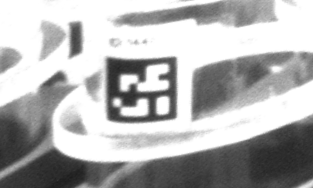
\includegraphics[width = \textwidth/3]{Bilder/cup2.png}
        \centering
    \end{figure}

    
    \begin{figure}
        \caption[Bildmatrixanalyse]{\small Bildmatrixanalyse am verzerrten optischen Marker.}\label{fig:figure21}
        \includegraphics[width = \textwidth]{Bilder/cup6_analyse.png}
        \centering
    \end{figure}

    \clearpage
    \lstinputlisting[language=Python, caption=Bildmatrixanalyse (Dateipfade gekürzt), label=Bildmatrixanalyse]{Listings/Bildmatrixanalyse_Becher6.py}
    \clearpage

    \subsection{Analyse der Erkennungsrate der Becher mittels Übersichtskamera}

    Die Bilder \ref{fig:figure12} bis \ref{fig:figure20} zeigen die Ergebnisse der Bildverarbeitungskette von der Aufnahme bis zur Bildsegmentierung und Erkennung.

    Die Bilder \ref{fig:figure22} bis \ref{fig:figure27} zeigen Überlegungen wie die Erkennung der Becher besser gelingen kann. 

    \begin{figure}
        \caption[Erkennungsrate der Becher ohne weitere Bildverabeitung]{\small Erkennungsrate der Becher ohne Bildbearbeitung.}\label{fig:figure22}
        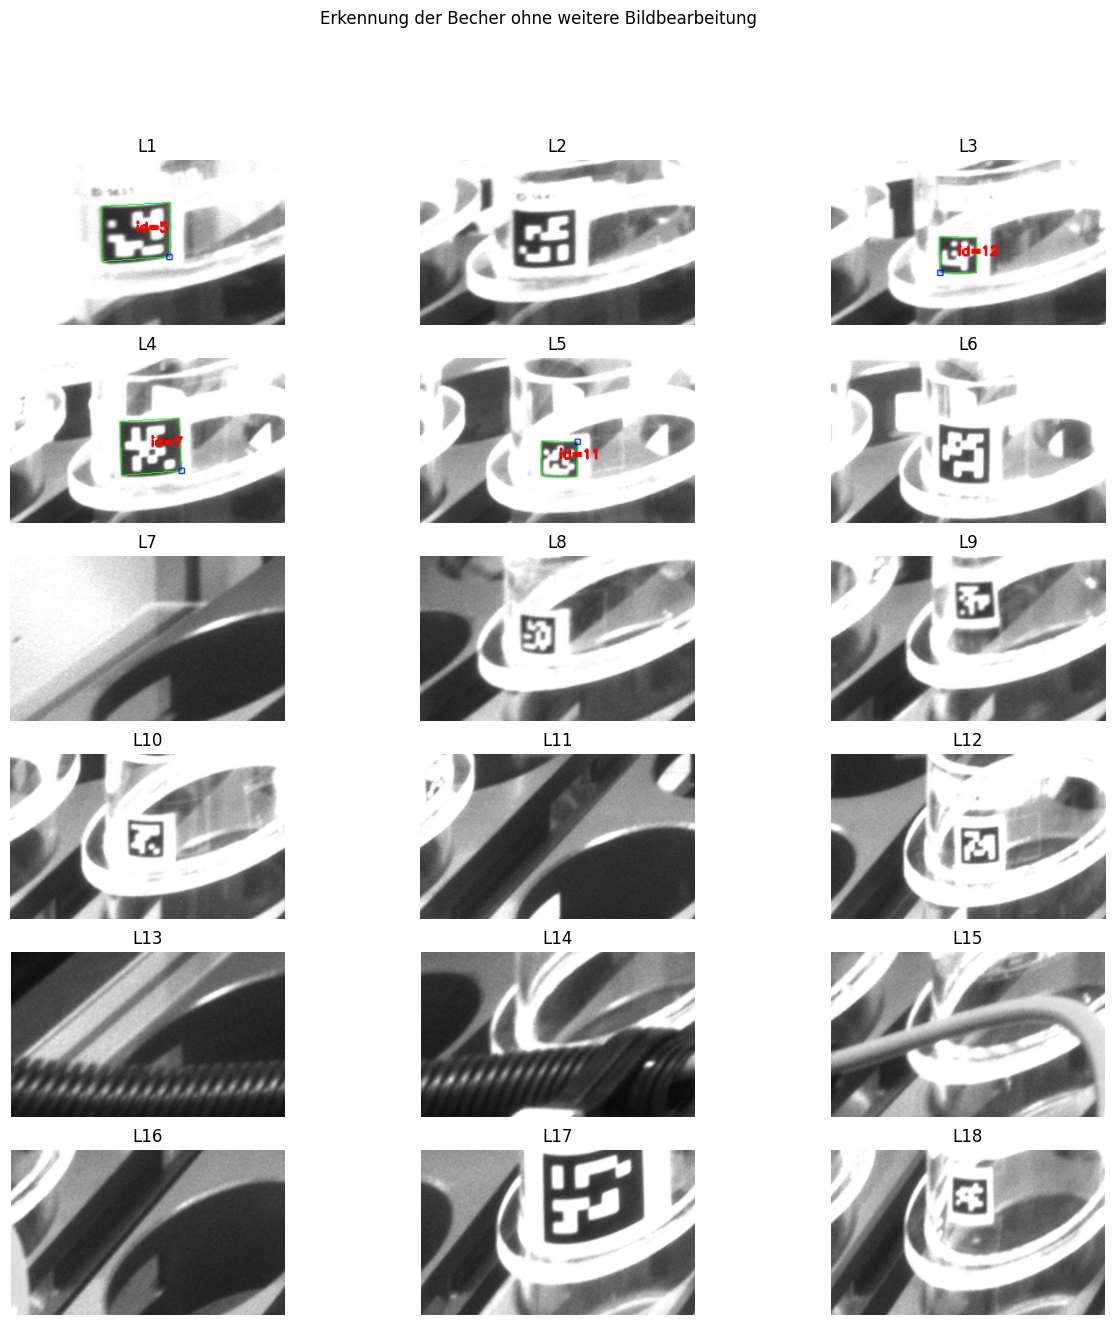
\includegraphics[width = \textwidth]{Bilder/ErkennungsrateOBB.png}
        \centering
    \end{figure}

    \begin{figure}
        \caption[Erkennungsrate nach Gauß 5x5 Filterung]{\small Erkennungsrate der Becher nach Gauß 5x5 Filterung.}\label{fig:figure23}
        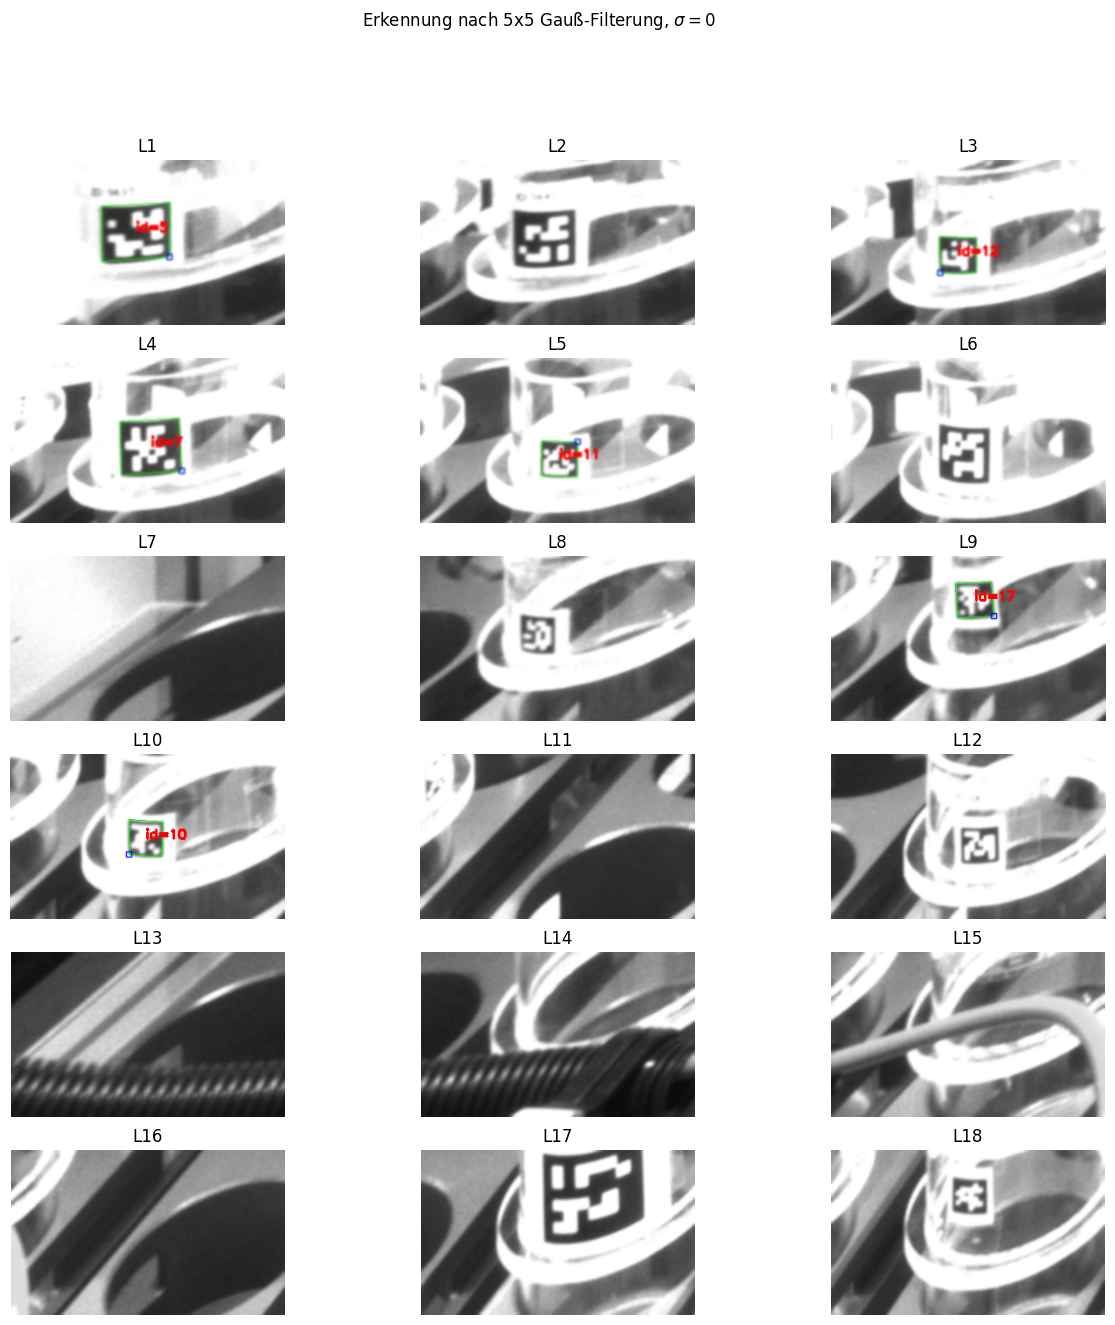
\includegraphics[width = \textwidth]{Bilder/ErkennungsrateGauss.png}
        \centering
    \end{figure}

    \begin{figure}
        \caption[Erkennungsrate nach Laplace Filterung]{\small Erkennungsrate der Becher nach Laplace Filterung.}\label{fig:figure24}
        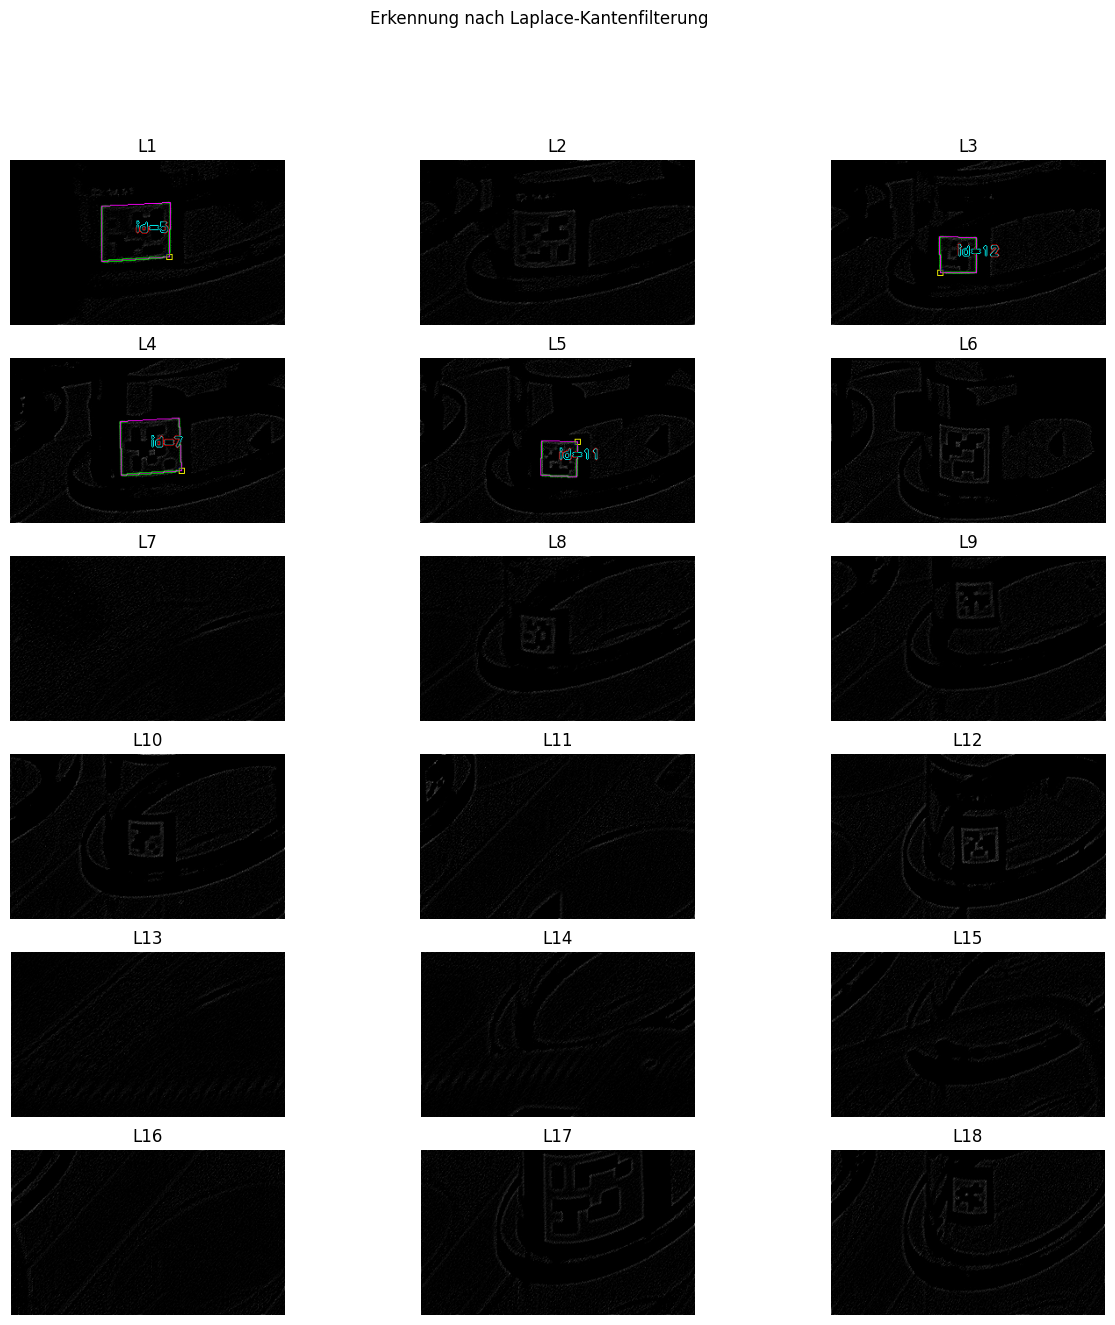
\includegraphics[width = \textwidth]{Bilder/ErkennungsrateLaplace.png}
        \centering
    \end{figure}

    \begin{figure}
        \caption[Erkennungsrate nach Überlagerung von Gauß und Laplace Filter]{\small Erkennungsrate der Becher nach Gauß 5x5 und Laplace Filterung (gewichtete Überlagerung).}\label{fig:figure25}
        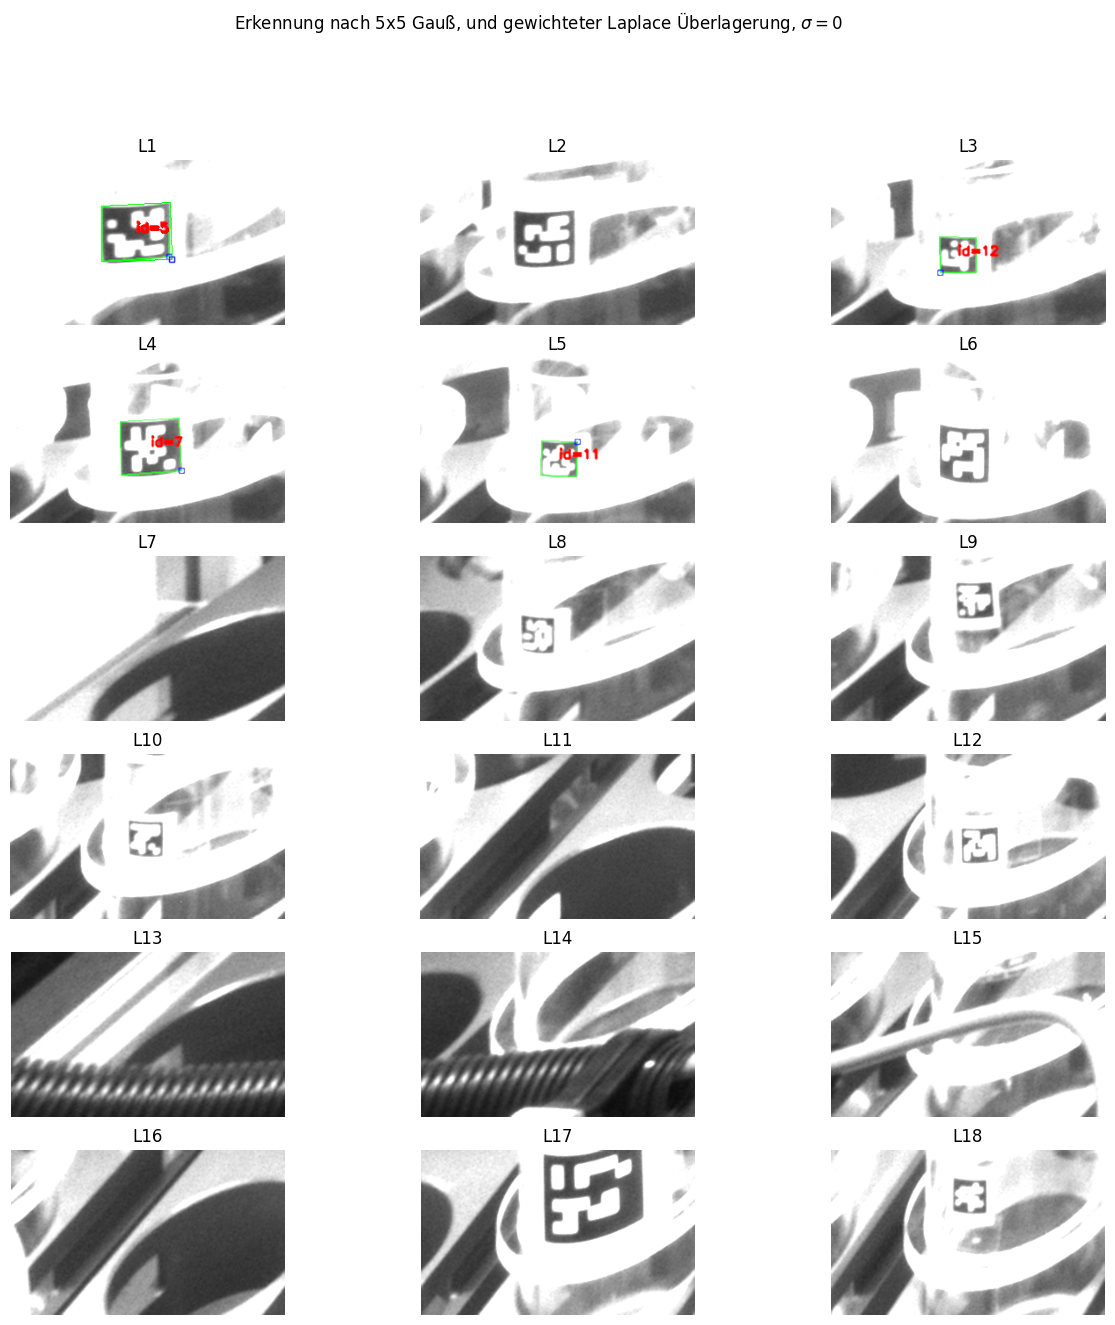
\includegraphics[width = \textwidth]{Bilder/ErkennungsrateGausLaplace.png}
        \centering
    \end{figure}

    \begin{figure}
        \caption[Erkennungsrate der Becher nach Schärfung und Gauß 5x5 Filterung]{Erkennungsrate der Becher nach Schärfung und anschließender Gauß 5x5 Filterung}\label{fig:figure26}
        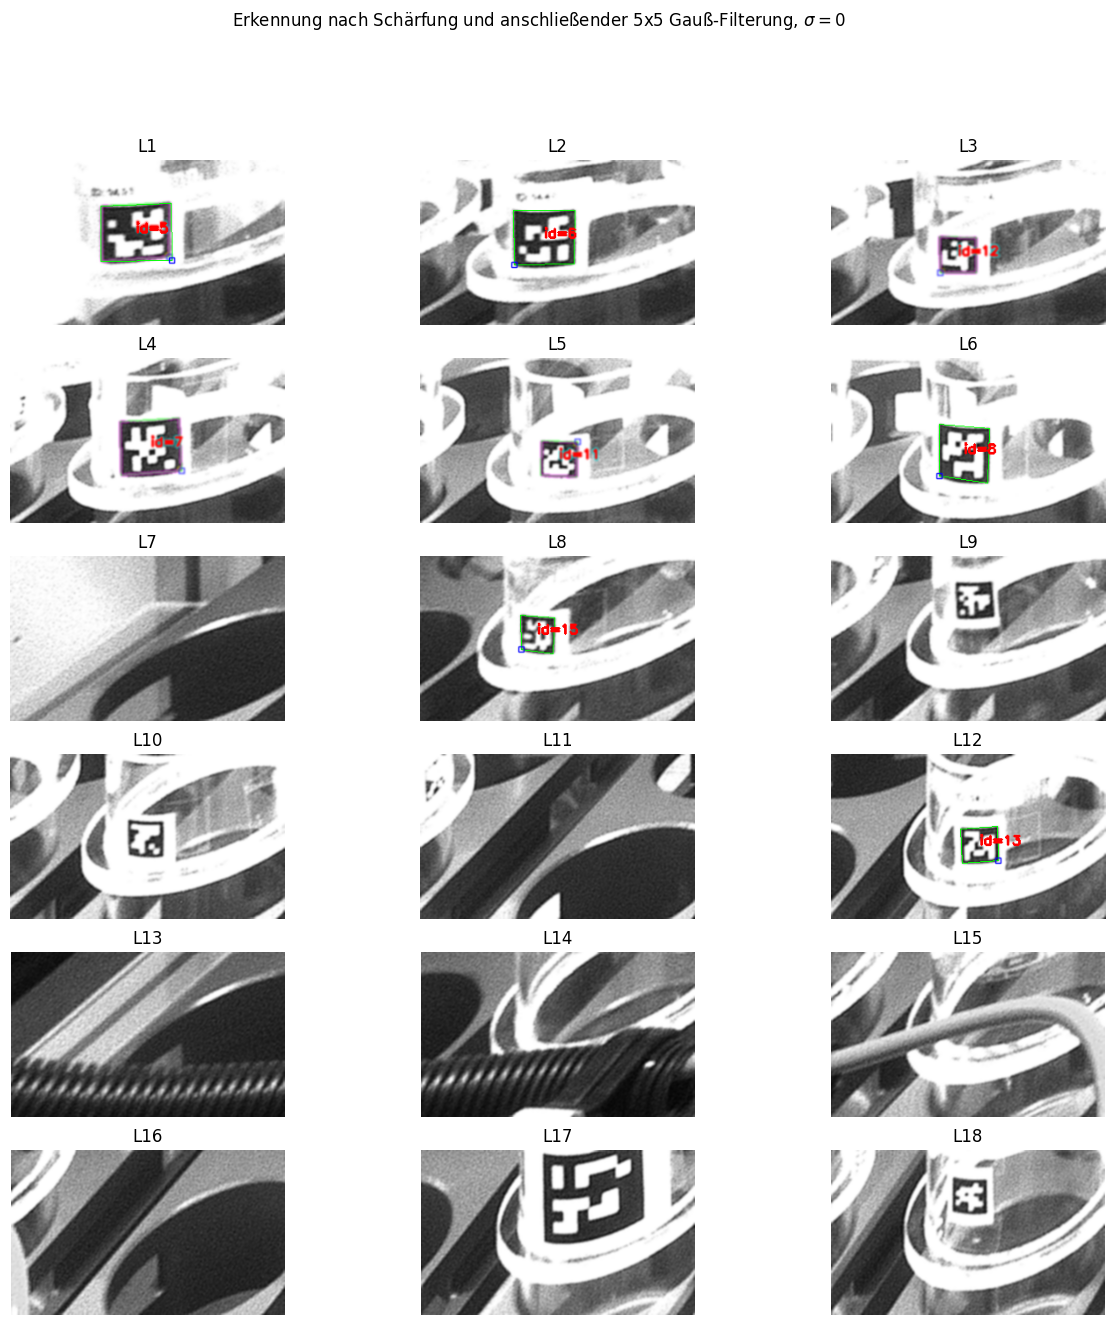
\includegraphics[width = \textwidth]{Bilder/ErkennungsrateScharfGauss.png}
        \centering
    \end{figure}

    Es wurden Versuche unternommen um die Erkennung mit systematischen Methoden zu verbessern.
    In \ref{fig:figure22} ist die Erkennungsrate der Becher ohne Bildbearbeitung dargestellt und dient somit als Referenz für die darauffolgenden Methoden der Bildverarbeitung.
    Es wurden 4 Marker korrekt erkannt, was durch das grüne Viereckt und der roten ID- Notiz erkennbar ist. 
    Es wurden zudem richtigerweise in den Plätzen L7, L11, L13, L14, L15 und L16 keine Becher erkannt.

    In \ref{fig:figure23} ist die Erkennungsrate nach einer Gauß 5x5 Filterung dargestellt. 
    Die Überlegung ist, dass durch das Reduzieren von Rauschen die Umwandlung von Graubild zu Binärbild dafür sorgt, dass die Binärmatrix gut genug dekodiert werden kann. 
    Wie in der Abbildung ersichtlich ist dies für L10 sogar der Fall - ansonsten ist jedoch keine Änderung des Ergebnisses ersichtlich.

    Der Versuch die Erkennung mit einem Laplace Kantenfilter zu verbessern, ist in \ref{fig:figure24} dargestellt und ergibt sogar eine schlechtere Erkennungsrate als das Referenzbild.
    
    In \ref{fig:figure25} ist die Erkennungsrate nach einer gewichteten Überlagerung von Gauß 5x5 und Laplace Filterung dargestellt. 
    Dazu wird zunächst ein mit einem Gauß 5x5 Filter gefiltertes Bild erzeugt und mit einem Laplace-Kantenbild überlagert. 
    Für die Überlagerung wird die Funktion \verb|cv2.addWeighted()| verwendet. 
    Durch die Überlagerung ergibt sich theoretisch ein höherer Kontrast der Kanten in der Binärmatrix. 
    Die Erkennungsrate ist jedoch nicht besser als die im Referenzbild.

    In \ref{fig:figure26} ist die Erkennungsrate nach einer Schärfung und anschließender Gauß 5x5 Filterung dargestellt.
    Für die Schärfung wurde die Filtermatrix $W$ verwendet, die mit 
    \begin{align*}
        W = \begin{bmatrix}
            -1 & -1 & -1 \\
            -1 & 9 & -1 \\
            -1 & -1 & -1
        \end{bmatrix}
    \end{align*}
    definiert ist. Allein das Schärfen des Bildes brachte keinen Erfolg. Nach der Gauß-Filterung steigt die Erkennungsrate auf 8 Marker an. 
    Die Marker L9, L10 und L18 werden nicht erkannt, was das Gesamtergebnis immer noch als zu unbefriedigend erscheinen lässt.

    Als Fazit der Versuche lässt sich festhalten, dass die Erkennung der Becher nicht mit einer zufriedenstellenden Sicherheit durch die verwendete Übersichtskamera durchführen lässt. 

    \subsection{Erkennungsrate der ESP32 Kamera}\label{ErkennungsrateESP32}

    Die ESP32 Kamera hat eine deutlich geringere Auflösung als die $\mu$Eye Kamera, hat aber einen sehr niedrigen Mindestabstand der Appertur.
    Um die Eignung der Kamera zu zeigen wurden 3 Testbilder aufgenommen, die in \ref{fig:figure27} dargestellt sind.

    Hier zeigt sich der Vergleich zu den vorangegangenen Abschnitten, dass die Erkennung der Marker selbst mit Wölbung kein Problem ist, wenn der Bildbereich und die Auflösung in einem günstigen Verhältnis stehen.
    Ohne weitere Bildverarbeitung werden die Marker im linken und rechten Bereich erkannt. 
    Das rechte Bild zeigt, dass bei der Anbringung und Größe der Marker Grenzen gesetzt sind: 
    Wenn der Rand der Binärmatrix außerhalb des Bildbereichs ist, wird der Marker nicht erkannt.

    \begin{figure}
        \caption[Testbilder mit ESP 32 WebCam]{Testbilder im Zuge der Positionsermittlugn für die ESP32 Kamera auf dem Greifer des IRB 140 Roboterarms.}\label{fig:figure27}
        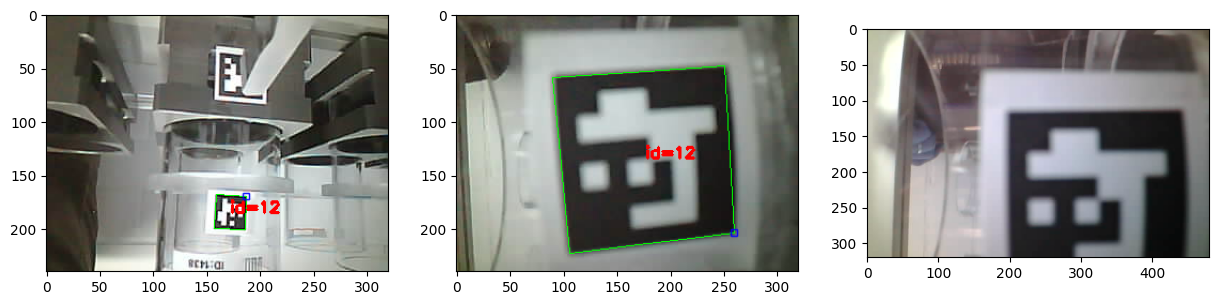
\includegraphics[width = \textwidth]{Bilder/ESP32CamTest.png}
        \centering
    \end{figure}

    \subsection{Festlegung der Markergröße und Position}

    Die Marker werden in folgende Gruppen unterschieden:
    \begin{itemize}
        \item Regalmarker
        \item Palettenmarker
        \item Bechermarker
    \end{itemize}
    Die Größe der Regalmarker hat sich mit 30x30mm bewährt ebenso die 6x6 Bit Binärmatrix, die Erkennungsrate ist ausreichend. die Wenigen Fehlschläge können in der Software abgefangen werden und eine neue Aufnahme anfordern.
    Die Palettenmarker sind mit einer Größe von 30x30 mm ebenfalls ausreichend. 
    Die Erkennung wird teilweise durch den Greifer verhindert, wenn dieser in Grundstellung ist. 
    Für die Palettenerkennung muss der Roboterarm daher die Grundstellung verlassen. 
    Eine Vergrößerung der Marker birgt das Risiko, dass Markerelemente den Bildbereich oder den Segmentbereich verlassen. 
    Eine Kleinere Markergröße verschlechtert die Erkennungsrate mit der Übersichtskamera enorm. 
    In den obigen Bildern wurde bspw. L18 nicht einmal erkannt.
    
    Die Erkennung der Becher mittels Übersichtkamera wird durch zwei Aspekte verhindert:
    \begin{itemize}
        \item Die Wölbung der Becher erschwert das Auslesen in Abhängigkeit von der Winkelposition des Bechers zur Kamera, siehe \ref{ChapBildmatrixanalyse}.
        \item Die vorderen Becher verdecken die hinteren Becher.
    \end{itemize}

    Daher erfolgt die Erkennung der Becher mittels ESP32 Kamera auf dem Greifer des Roboterarms.
    Günstige Gelegenheiten ohne nennenswerte Störung des Betriebsablaufs sind gegeben, bevor der Roboter einen Becher oder Palette greift.
    In diesen Situationen blickt die Kamera mittig und rechtwinklig auf den Bechermantel, wie \ref{fig:figure27} veranschaulicht.

    Um die Erkennnung der Marker zu gewährleisten, muss um den Rand des Markers ein \glqq Ruhebereich \grqq von wenigen Millimetern eingehalten werden.
    Dies trifft insbesondere auf die Palettenmarker zu, da die Paletten ein dunkles Grau haben und die Unterscheidung zum Marker bei ungünstigen Lichtverhältnissen unmöglich macht.
    Das Drucken der Marker mit schwarzem Toner auf weißem Druckerpapier ist ausreichend.


